\documentclass[defaultstyle,10pt,master,Helvetica]{01.thesis}
% Helvetica is a similar font to Arial, with small differences.

%% Packages
\typeout{}
\typeout{--------------------------------------------------------------}
\typeout{ +---+ Thesis Template                            }
\typeout{ +---+      Version 2.0, November 2017                         }
\typeout{ +---+  for Instituto Superior Tecnico (IST),                 }
\typeout{ +---+  Universidade Técnica de Lisboa                         }
\typeout{ * Using Thesis Style from Pedro Tomás                                }
\typeout{ * Created to write Dissertations                             }
\typeout{ * Conforms with IST Doctoral Degree format and with most important packages setup        }
%\typeout{ * Should conform with IST PhD Degree format (not verified)   }
\typeout{                                                              }
\typeout{ AUTHOR: Filipe Marques; (original Master Degree Thesis Template authors:) Miguel Amador and João Marques                                          }
\typeout{                                                              }
\typeout{Important: Use all files in the archive, since this is based in all them. Modify dummy files at wish.                                                              }
\typeout{--------------------------------------------------------------}
\typeout{}

% Defines an additional alphabet... not required in most cases
% ------------------------------------------------------------
% \DeclareMathAlphabet{\mathpzc}{OT1}{pzc}{m}{it}

% PACKAGE babel:
% ---------------
% The 'babel' package may correct some hyphenisation issues of latex. 
% However in most situations it is not required.
\usepackage[english,portuguese]{babel}


% PACKAGE fontenc:
% -----------------
% chooses T1-fonts and allows correct automatic hyphenation.
%\usepackage[T1]{fontenc}
%\usepackage[latin1]{inputenc}
\usepackage[utf8]{inputenc}
\usepackage[T1]{fontenc}
%\usepackage{lmodern} %will change font type

% Package ulem.
\usepackage{ulem} % Allows the use of other text emphatizer commands
\normalem %defines \emph{} to italic, instead of underline. 
\raggedbottom %declaration makes all pages the height of the text on that page. No extra vertical space is added. The \flushbottom declaration makes all text pages the same height, adding extra vertical space when necessary to fill out the page.

% PACKAGE date time:
% -----------------
% Lets you alter the format of the date that \today returns.
\usepackage{datetime}
\newdateformat{todaythesis}{%
\monthname[\THEMONTH]  \THEYEAR}

% PACKAGE latexsym:
% -----------------
% Defines additional latex symbols. May be required for thesis with many math symbols.
\usepackage{latexsym}

% MATH PACKAGES amsthm, amssymb, amsfonts...:
% -------------------------------------------
% This package is typically required. Among many other things it adds the possibility
% to put symbols in bold by using \boldsymbol (not \mathbf); defines additional 
% fonts and symbols; adds the \eqref command for citing equations. I prefer the style
% "(x.xx)" for referering to an equation than to use "equation x.xx".
\usepackage{amsthm, amssymb, amsfonts, amsbsy}
\usepackage{mathtools}%The mathtools package fixes some amsmath quirks and adds some useful settings, symbols, and environments to amsmath.
\usepackage{xcolor,cancel} % xcolor to change the texto color; cancel to use a cancel line in equations.
%https://en.wikibooks.org/wiki/LaTeX/Colors

% PACKAGE TABLES multirow, colortbl, longtable:
% ---------------------------------------
% These packages are most usefull for advanced tables. The first allows to join rows 
% throuhg the command \multirow which works similarly with the command \multicolumn
% The second package allows to color the table (both foreground and background)
% The third package is only required when tables extend beyond the length of one page;
% with compatibilities with the tabular environment. The last allow the definitions of landscape pages, allowing the use of a different orientation for wider graphics or tables. See package documentation to see the implementation.
\usepackage{multirow}
\usepackage{colortbl}
\usepackage{supertabular}
\usepackage{pdflscape}
% \usepackage{longtable}
\usepackage{tabularx}	% (default: necessary for the cover)
\usepackage{longtable,tabu}

% PACKAGE GRAPHICS graphics, epsfig, caption, etc...:
% ---------------------------------------------
% Packages for figures... well you will certainly need these packages, with the exception
% of the 'caption' package. This only allows to define extra caption options.
% Notice that subfigure allows to place figures within figures with its own caption. It
% should be avoided to create an eps file with subfigures. That will mean that you won't be 
% able to reference those subfigures. Instead create an EPS file (the only graphics format supported
% by latex) for each of the subfigures and then use the command \subfigure (see below).
\usepackage{graphics}
\usepackage{graphicx}
%\usepackage[pdftex]{graphicx} %> esta selecção provoca colisão com epsfig e caption...
\usepackage{epsfig}	%colisao com graphicx
\usepackage[font=small,labelfont=bf,textfont=normalfont]{caption}
\usepackage{caption} 	%to alter captions  (\usepackage[footnotesize,bf,center]{caption})
%\usepackage[hang,small,bf]{subfigure} %deprecated > use subfig or subcaption:
\usepackage{subcaption}	%for subfigures
\usepackage{dcolumn}
\usepackage{bm}
\usepackage{booktabs}
\usepackage{rotating}
\usepackage{multirow}				%colisao com graphicx

\usepackage{color}% to alter text colour
\usepackage{pstricks} % to inkscape latex... not working
\usepackage{import} %to pdf-tex import from different place

\usepackage{pdfpages} %annex pdf pages

% PACKAGE algorithmic, algorithm
% ------------------------------
% These packages are required if you need to describe an algorithm.
% \usepackage{algorithmic}
% \usepackage[chapter]{algorithm}

% PACKAGE natbib/cite/biblatex
% -------------------
% The three packages are not compatible, and you should use one of the two. Notice however that the
% IEEE BiBTeX stylesheet is imcompatible with the natbib package. If using the IEEE format, use the 
% cite package instead
%% Natbib
\usepackage[square,numbers,sort&compress]{natbib}
%% Cite
%\usepackage{cite}
%% Biblatex (Not working)
%\usepackage{csquotes}
%\usepackage[backend=biber,style=authoryear]{biblatex}


% PACKAGE acronyum
% -----------------
% This package is most useful for acronyms. The package guarantees that all acronyms definitions are 
% given at the first usage. IMPORTANT: do not use acronyms in titles/captions; otherwise the definition 
% will appear on the table of contents.
\usepackage[printonlyused]{acronym}
\usepackage[titletoc,title,header]{appendix}
\usepackage[noauto]{chappg}
%The following line assures that each chapter deals with acronyms independently.
%You may also do it manually by calling acresetall anywhere in the documento to reset the acronyms behaviour. 
\preto\chapter\acresetall

% PACKAGE extra_functions VER COMO DEVE SER
% -----------------
% My Personal package: defines the following commands:
% \fancychapter{chaptername) -> Prints a fancier chapter (you can also use the fancychapter package for this)
% \hline{width} -> use for a replacement of the \hline command
% \Mark1, \Mark2, \Mark3, ...
\usepackage{00.extra_functions}


% PACKAGE hyperref
% -----------------
% Set links for references and citations in document
% Some MiKTeX distributions have faulty PDF creators in which case this package will not work correctly
% Long live Linux :D
\usepackage[plainpages=false]{hyperref}
\hypersetup{
             colorlinks=false,
             citecolor=red,
             breaklinks=true,
             bookmarksnumbered=true,
             bookmarksopen=true,
             pdftitle={Thesis Title},
             pdfauthor={Author Name},
             pdfsubject={Doctoral Thesis in Mechanical Engineering},
             pdfcreator={Document Creator Name},
             pdfkeywords={Template, Latex, Thesis}}
%\usepackage[pdftex,bookmarks,colorlinks,breaklinks]{hyperref}  % PDF hyperlinks, with coloured links
%%\hypersetup{linkcolor=blue}
%\hypersetup{linkcolor=black}
\usepackage{float}
%\usepackage[final]{00.listofsymbols}
\usepackage{00.symlist}

% Set paragraph counter to alphanumeric mode
\renewcommand{\theparagraph}{\Alph{paragraph}~--}

\usepackage{enumitem}	% para set list
\usepackage{algpseudocode} % algorithmic pseudocode
\usepackage[chapter]{algorithm}

\usepackage{scrextend}
\usepackage{marginnote}%temporary notes at the margin
\usepackage{multicol} %multiple columns environment
%solves figure problem: http://tex.stackexchange.com/questions/12262/multicol-and-figures
\newenvironment{Figure}
  {\par\medskip\noindent\minipage{\linewidth}}
  {\endminipage\par\medskip}

\usepackage{siunitx}
\sisetup{load-configurations = abbreviations}
%%% -------------------- declares extra units
\DeclareSIUnit\Mtoe{\mega \tonne oe} % use: \SI{100}{\Mtoe}
\DeclareSIUnit\GWh{GWh} % use: \SI{100}{\GWh}  (not \GW\hour = GW h )
%%% -------------------------------------------------

 \usepackage{wrapfig} % to wrap text around small figures
 \usepackage{chemformula} % for chemical formulae : http://mirrors.fe.up.pt/pub/CTAN/macros/latex/contrib/chemformula/chemformula_en.pdf
 \usepackage{dcolumn} %dcolumns in tables : https://en.wikibooks.org/wiki/LaTeX/Tables#Defining_multiple_columns

%%%%%%%%%%%%   glossaries
\usepackage{makeidx} %necessary?
\usepackage[acronym,xindy]{glossaries} %adicionar nomain option para evitar a impressão do glossário main em caso de engano, adicionar nonumberlist
%\usepackage[nomain,acronym,makeindex]{glossaries}
%\usepackage{glossary-mcols} % em colunas
%\setglossarystyle{mcolindex} %estilos de glossário, ver documentação
%\setacronymstyle{long-short}
\loadglsentries{./00.Definitions/Notation-List.tex} % loads list, needs to be in the preamble
\loadglsentries{./00.Definitions/Acronyms-List.tex} % loads list

\makeglossaries

%% change to setglossarystyle
\newglossarystyle{mylist}{% 
\glossarystyle{index}% base this style on the list style 
%\renewcommand{\glsgroupskip}{}% make nothing happen between groups 
\renewenvironment{index}% 
    {\tablehead{}\tabletail{}% 
     \begin{supertabular}{lp{\glsdescwidth}}}% 
    {\end{supertabular}}% 
} 
%%%%%%%%%%%%




%% Page formatting
\hoffset 0in
\voffset 0in

%Alternative set of page geometry
%\oddsidemargin 0.71cm
%\evensidemargin 0.04cm
%\marginparsep 0in
%\topmargin -0.25cm
%\textwidth 15cm
%\textheight 23.5cm

\usepackage[top=2.5cm, bottom=2.5cm, inner=2.9cm, outer=2.5cm]{geometry}

\usepackage{fancyhdr}
\pagestyle{fancy}
\renewcommand{\chaptermark}[1]{\markboth{\thechapter.\ #1}{}}
\renewcommand{\sectionmark}[1]{\markright{\thesection\ #1}}
\fancyhf{} 
%\fancyhead[LE]{\bfseries\nouppercase{\leftmark}}
%\fancyhead[RO]{\bfseries\nouppercase{\rightmark}}
\fancyfoot[LE,RO]{\bfseries\small\thepage}
\renewcommand{\headrulewidth}{0.0pt}
\renewcommand{\footrulewidth}{0.0pt}
\addtolength{\headheight}{2pt} % make space for the rule
\fancypagestyle{plain}{% Used in Chapter titles
   \fancyhead{} % get rid of headers
   \renewcommand{\headrulewidth}{0pt} % and the line
   \renewcommand{\footrulewidth}{0pt}
   \fancyfoot[LE,RO]{\bfseries\small\thepage}
}

\fancypagestyle{begin}{%
   \fancyhead{}
   \renewcommand{\headrulewidth}{0pt}
   \renewcommand{\footrulewidth}{0pt}
   \fancyfoot[LE,RO]{\bfseries\small\thepage}
}
\fancypagestyle{document}{%
	\fancyhf{} 
	\fancyhead[LE]{\bfseries\nouppercase{\leftmark}}
	\fancyhead[RO]{\bfseries\nouppercase{\rightmark}}
	\fancyfoot[LE,RO]{\bfseries\small\thepage}
	%\renewcommand{\headrulewidth}{0pt}
	%\renewcommand{\footrulewidth}{0pt}
	\addtolength{\headheight}{2pt} % make space for the rule
}
\fancypagestyle{documentsimple}{%
	\fancyhf{}
	\fancyfoot[LE,RO]{\bfseries\small\thepage}
	%\renewcommand{\headrulewidth}{0pt}
	%\renewcommand{\footrulewidth}{0pt}
	\addtolength{\headheight}{2pt} % make space for the rule
}
\setcounter{secnumdepth} {5}
\setcounter{tocdepth} {5}
\renewcommand{\thesubsubsection}{\thesubsection.\Alph{subsubsection}}

\renewcommand{\subfigtopskip}{0.3 cm}
\renewcommand{\subfigbottomskip}{0.2 cm}
\renewcommand{\subfigcapskip}{0.3 cm}
\renewcommand{\subfigcapmargin}{0.2 cm}

\graphicspath{{Figures/}}



%-----------------------------------------------------------
%-----------------------------------------------------------
\begin{document}
\pagestyle{begin}
\setcounter{page}{1} \pagenumbering{Alph}

% Add PDF bookmark 
\pdfbookmark[0]{Title}{Title}

\thispagestyle{empty}
\begin{flushleft} ~\\ \vspace{-12mm} \hspace{-12mm}  
\includegraphics[width=50mm]{Cover/istnewlogo} 
\vspace{10mm}
%~\\ \vspace{50mm} % gr�ficos
\\ \begin{center} 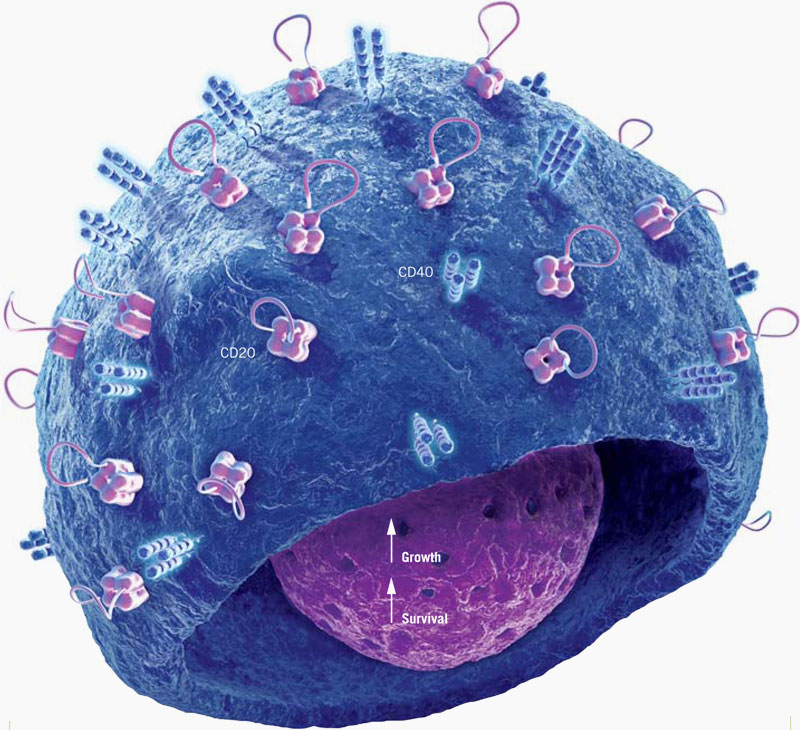
\includegraphics[height=50mm]{Cover/coverimage}  \end{center} % gr�ficos
 \vspace{5mm}
\centering
\LARGE \textbf{Thesis Title}
\\ \vspace{10mm}
\Large Subtitle
\\ \vspace{15mm}
\Large \textbf{Full Name} \\
\vspace{12mm}
\large Thesis to obtain the Master of Science Degree in
\\ \vspace{2mm}
\LARGE \textbf{Biomedical Engineering}
\\ \vspace{10mm}
\large Supervisor(s): Prof./Dr. Lorem Ipsum
\\ \vspace{15mm}
\Large \textbf{Examinatiom Committee}
\\ \vspace{5mm}
\large Chairperson:	Prof. Lorem \\
\large Supervisor: Prof. Lorem Ipsum\\
\large Co-Supervisor: Prof. Lorem Ipsum \\
\large Members of the Committe: Dr. Lorem Ipsum \\
Prof. Lorem Ipsum
 
\vspace{15mm}

%\Large \textbf{\todaythesis\today} \\
\Large \textbf{January 2015} \\
\let\thepage\relax
\end{flushleft}
\pagebreak


\clearpage
% Since I am using double sided pages, the second page should be white.
% Remember that when delivering the dissertation, IST requires for the cover to appear twice.

\thispagestyle{empty}
\cleardoublepage

\setcounter{page}{1} \pagenumbering{roman}

\baselineskip 18pt % line spacing: -12pt for single spacing
                   %               -18pt for 1 1/2 spacing
                   %               -24pt for double spacingnts} 
\thispagestyle{empty}
\hbox{} \vfill
\begin{flushright}
\small \textit{\textbf{Anyone who has never made a mistake has never tried anything new.}}
\\ \vspace{2mm}  
\scriptsize Albert Einstein
\end{flushright}

\clearpage
\thispagestyle{empty}
\cleardoublepage

\pdfbookmark{Acknowledgments}{Acknowledgments}
\begin{acknowledgments} 

I would like to thank the Academy, bla bla bla..

\end{acknowledgments}
\clearpage
\thispagestyle{empty}
\cleardoublepage
\begin{abstract}

The Objective of this Work ... (English)

\end{abstract}
\begin{keywords}
Keywords (English)
\end{keywords}
\clearpage
\thispagestyle{empty}
\cleardoublepage
\begin{resumo}

O objectivo deste trabalho ... (Português)

\end{resumo}
\begin{palavraschave}
Palavras-Chave (Português)
\end{palavraschave}
\clearpage
\thispagestyle{empty}
\cleardoublepage
% This is required for the fancy chapters
\dominitoc
\dominilof
\dominilot

%%%%%%%%%%%%%%%%%%%%%%%%%%%%%%%%%%%%%%%%%%%%%%%%%%%%%%%%%%%%%%%%%%%%%%
% List of contents
%\renewcommand{\baselinestretch}{1}
\pdfbookmark[0]{Index}{index}
\pdfbookmark[1]{Contents}{toc}
\tableofcontents
% \contentsline{chapter}{References}{\pageref{bib}}
\clearpage
\thispagestyle{empty}
\cleardoublepage
%\renewcommand{\baselinestretch}{1.5}
%%%%%%%%%%%%%%%%%%%%%%%%%%%%%%%%%%%%%%%%%%%%%%%%%%%%%%%%%%%%%%%%%%%%%%
% List of figures
\pdfbookmark[1]{List of Figures}{lof}
\listoffigures
\clearpage
\thispagestyle{empty}
\cleardoublepage

%%%%%%%%%%%%%%%%%%%%%%%%%%%%%%%%%%%%%%%%%%%%%%%%%%%%%%%%%%%%%%%%%%%%%%
% List of tables
\pdfbookmark[1]{List of Tables}{lot}
\listoftables
\clearpage
\thispagestyle{empty}
\cleardoublepage

% %%%%%%%%%%%%%%%%%%%%%%%%%%%%%%%%%%%%%%%%%%%%%%%%%%%%%%%%%%%%%%%%%%%%%%
% % List of algorithms
% Requires packages algorithmic, algorithm
% \pdfbookmark[1]{List of Algorithms}{loa}
% \listofalgorithms
% \cleardoublepage
\acresetall
% %%%%%%%%%%%%%%%%%%%%%%%%%%%%%%%%%%%%%%%%%%%%%%%%%%%%%%%%%%%%%%%%%%%%%%
 % List of acronyms
\pdfbookmark[1]{List of Acronyms}{loac}

\chapter*{Abbreviations}


% See more at http://staff.science.uva.nl/~polko/HOWTO/LATEX/acronym.html

\begin{acronym}
\acro{acro}{Dummy Acronym}
\end{acronym}

\clearpage
\thispagestyle{empty}
\cleardoublepage




%%%%%%%%%%%%%%%%%%%%%%%%%%%%%%%%%%%%%%%%%%%%%%%%%%%%%%%%%%%%%%%%%%%%%%
% List of symbols
\pdfbookmark[1]{List of Symbols}{los}

\listofsymbols

\clearpage
\thispagestyle{empty}

\cleardoublepage
% Pages number is starting now with arabic style... until now it was on roman mode
\pagenumbering{arabic} \setcounter{page}{1}
\baselineskip 18pt
%\pagestyle{document}%Fancy head and foot with lines
\pagestyle{documentsimple}%Simple head
% %%%%%%%%%%%%%%%%%%%%%%%%%%%%%%%%%%%%%%%%%%%%%%%%%%%%%%%%%%%%%%%%%%%%%%
% The Introduction:
% %%%%%%%%%%%%%%%%%%%%%%%%%%%%%%%%%%%%%%%%%%%%%%%%%%%%%%%%%%%%%%%%%%%%%%
\fancychapter{Introduction}
\label{cap:int}

\section{Motivation}
\label{sec:int_motivation}

Motivation Section.
\section{State of The Art}
\label{sec:int_state}

State of The Art Section.

\subsection{Dummy Subsection A}
\label{subsec:subsectiona}

State of Art Subsection A

\subsection{Dummy Subsection B}
\label{subsec:subsectionb}

State of Art Subsection B


\section{Original Contributions}
\label{sec:int_contributions}

Contributions Section.
\section{Thesis Outline}
\label{sec:int_outline}

Outline Section.

\cleardoublepage
% %%%%%%%%%%%%%%%%%%%%%%%%%%%%%%%%%%%%%%%%%%%%%%%%%%%%%%%%%%%%%%%%%%%%%%
% Dummy Chapter:
% %%%%%%%%%%%%%%%%%%%%%%%%%%%%%%%%%%%%%%%%%%%%%%%%%%%%%%%%%%%%%%%%%%%%%%

% %%%%%%%%%%%%%%%%%%%%%%%%%%%%%%%%%%%%%%%%%%%%%%%%%%%%%%%%%%%%%%%%%%%%%%
% The Introduction:
% %%%%%%%%%%%%%%%%%%%%%%%%%%%%%%%%%%%%%%%%%%%%%%%%%%%%%%%%%%%%%%%%%%%%%%
\fancychapter{A Chapter}
\label{cap:chapter}

\textit{Present the chapter content.}

\section{Section A}
\label{sec:sectiona}

\subsection{Subsection A}
\label{subsec:subasectionA}

This would be a citation \cite{dummy}.

The \gls{cop} defines the performance of the machine.
% The first time you use this, the acronym will be written in full with the acronym in parentheses: supernova (SN). At later times it will just print the acronym: SN.

Heat Pump's performance is given by the \gls{cophp}, a \gls{cop} for heat pumps.

Now, an example on notation: \gls{Eu} and \gls{slip}.
Also \gls{Cd}.

As seen in \cite{wiki}. \emph{Enfatizar}

\subsection{Subsection B}
\label{subsec:subbsectiona}

\begin{figure}[H]
	\centering
		
\includegraphics[width=0.5\linewidth]{2.Chapter/dummy.pdf}
	\caption[Dummy Figure Caption for List of Figures.]{Dummy Figure Caption.}
	\label{fig:dummyfigure1}
\end{figure}

Remember you can change the reference style. Another dummy citation \cite{site}.
\section{Section B}
\label{sec:sectionb}

\subsection{Subsection A}
\label{subsec:subasectionB}

The model described can also be represented as

\begin{equation}
\dot{\mathbf{x}}(t) = \mathbf{T}\mathbf{z}(y),\  \mathbf{y}(0) = \mathbf{y}_0,\  z\geq 0 \\
\label{eq:dummyeq1}
\end{equation}

\noindent where

\begin{equation}
\mathbf{A} = \left[ \begin{array}{cc} -(a_{12} + a_{10}) & a_{21} \\ a_{12} & -(a_{21} + a_{20}) \end{array} \right],\ \mathbf{x} = \left[ \begin{array}{c} x_1 \\ x_2 \end{array} \right] \\
\label{eq:dummyeq2}
\end{equation}

Also, using glossaries in the math environment, you can write
\begin{equation}
\gls{A} = \frac{\gls{mflow}\gls{_v}}{\rho u}
\label{eq:dummyeq3}
\end{equation}

Note that \gls{A} is not \gls{a}.


\subsection{Subsection B}
\label{subsec:subbsectionB}

Another example for the notation section: think about \gls{gamma}.
And \gls{gamma}\gls{_p} with a subscript.

\begin{table}[H]
	\centering
	\caption{Dummy Table.}
	\begin{tabular}{|c|c|c|c|} \hline
		\textbf{Vendor Name} 				& \textbf{Short Name}	& \textbf{Commercial Name}	& \textbf{Manufacturer}	\\ \hline \hline
		\multirow{3}{*}{Text in Multiple Row}		&	ABC				&  ABC\textreg				& ABC SA			         \\ \cline{2-4}
		 								&        DEF				&  DEF\textreg				& DEF SA				\\ \cline{2-4}
										&        GHF			&  GHF\textreg				& GHF SA				\\ \hline
		Text in Single Row					&        IJK				& IJK\textreg				& IJK SA				\\ \hline
		Frescos SA						&        LMN			& LMN\textreg				& LMN SA				\\ \hline
		Carros Lda.						&    \multicolumn{3}{|c|}{Text in Multiple Column}							\\ \hline
	\end{tabular}
	\label{tab:dummytable}
\end{table}
\cleardoublepage



% %%%%%%%%%%%%%%%%%%%%%%%%%%%%%%%%%%%%%%%%%%%%%%%%%%%%%%%%%%%%%%%%%%%%%%
% The Introduction:
% %%%%%%%%%%%%%%%%%%%%%%%%%%%%%%%%%%%%%%%%%%%%%%%%%%%%%%%%%%%%%%%%%%%%%%
\fancychapter{Conclusions and Future Work}
\label{cap:conclusions}

Conclusions Chapter

\cleardoublepage
\cleardoublepage
\phantomsection
\addcontentsline{toc}{chapter}{Bibliography}
\bibliographystyle{IEEEtran}
\bibliography{02.biblio}
\cleardoublepage

\begin{appendices}
	\begin{appendix}
		\pagenumbering{bychapter}
		\fancychapter{Title of AppendixA}
\label{ap:a}

   
		\cleardoublepage
	\end{appendix}
\end{appendices}


\end{document}